\documentclass[]{article}
\usepackage{lmodern}
\usepackage{amssymb,amsmath}
\usepackage{ifxetex,ifluatex}
\usepackage{fixltx2e} % provides \textsubscript
\ifnum 0\ifxetex 1\fi\ifluatex 1\fi=0 % if pdftex
  \usepackage[T1]{fontenc}
  \usepackage[utf8]{inputenc}
\else % if luatex or xelatex
  \ifxetex
    \usepackage{mathspec}
    \usepackage{xltxtra,xunicode}
  \else
    \usepackage{fontspec}
  \fi
  \defaultfontfeatures{Mapping=tex-text,Scale=MatchLowercase}
  \newcommand{\euro}{€}
\fi
% use upquote if available, for straight quotes in verbatim environments
\IfFileExists{upquote.sty}{\usepackage{upquote}}{}
% use microtype if available
\IfFileExists{microtype.sty}{%
\usepackage{microtype}
\UseMicrotypeSet[protrusion]{basicmath} % disable protrusion for tt fonts
}{}
\usepackage[margin=1in]{geometry}
\usepackage{graphicx}
\makeatletter
\def\maxwidth{\ifdim\Gin@nat@width>\linewidth\linewidth\else\Gin@nat@width\fi}
\def\maxheight{\ifdim\Gin@nat@height>\textheight\textheight\else\Gin@nat@height\fi}
\makeatother
% Scale images if necessary, so that they will not overflow the page
% margins by default, and it is still possible to overwrite the defaults
% using explicit options in \includegraphics[width, height, ...]{}
\setkeys{Gin}{width=\maxwidth,height=\maxheight,keepaspectratio}
\ifxetex
  \usepackage[setpagesize=false, % page size defined by xetex
              unicode=false, % unicode breaks when used with xetex
              xetex]{hyperref}
\else
  \usepackage[unicode=true]{hyperref}
\fi
\hypersetup{breaklinks=true,
            bookmarks=true,
            pdfauthor={JcB},
            pdftitle={Rapport 2014 - version FEDORU},
            colorlinks=true,
            citecolor=blue,
            urlcolor=blue,
            linkcolor=magenta,
            pdfborder={0 0 0}}
\urlstyle{same}  % don't use monospace font for urls
\setlength{\parindent}{0pt}
\setlength{\parskip}{6pt plus 2pt minus 1pt}
\setlength{\emergencystretch}{3em}  % prevent overfull lines
\setcounter{secnumdepth}{5}

%%% Use protect on footnotes to avoid problems with footnotes in titles
\let\rmarkdownfootnote\footnote%
\def\footnote{\protect\rmarkdownfootnote}

%%% Change title format to be more compact
\usepackage{titling}

% Create subtitle command for use in maketitle
\newcommand{\subtitle}[1]{
  \posttitle{
    \begin{center}\large#1\end{center}
    }
}

\setlength{\droptitle}{-2em}
  \title{Rapport 2014 - version FEDORU}
  \pretitle{\vspace{\droptitle}\centering\huge}
  \posttitle{\par}
  \author{JcB}
  \preauthor{\centering\large\emph}
  \postauthor{\par}
  \predate{\centering\large\emph}
  \postdate{\par}
  \date{28/01/2015}



\begin{document}

\maketitle


{
\hypersetup{linkcolor=black}
\setcounter{tocdepth}{2}
\tableofcontents
}
\section{Activité des structures d'urgences : panorama 2014 de la région
ALSACE}\label{activite-des-structures-durgences-panorama-2014-de-la-region-alsace}

Rapport 2014 respectant les préconisations de la FEDORU. Source:
\href{https://docs.google.com/document/d/101LYVqVLeHZnrujfMm3aqBYfbOwx3CPEB3Y-Lbud2Ls/edit}{Trame
commune}

Le document de référence pour le rapport est: \textbf{V4 trame commune
2014 rapport inter région} (xps:
/home/jcb/Documents/Resural/FEDORU/Trame\_Commune/DOC/Trame commune 2014
rapport inter région (V4).docx)

\textbf{NOTE}: certaines informations utiles sont dans
\textbf{RPU\_Doc}.

\section{LE MOT DU PRÉSIDENT DE LA
FEDORU}\label{le-mot-du-president-de-la-fedoru}

La publication du panorama des urgences de la région
\textbf{ALSACE}constitue une excellente occasion pour présenter la
fédération des observatoires régionaux des urgences (FEDORU) qui compte
\textbf{RESURAL} parmi ses membres actifs.

La FEDORU a été créée au mois d'octobre 2013. Ses membres sont chargés
dans leur région respective du traitement des données d'urgences ; ce
point commun est le trait d'origine de la FEDORU et donne son empreinte
à l'objet de notre association que je cite ici :

\begin{itemize}
\itemsep1pt\parskip0pt\parsep0pt
\item
  promouvoir les observatoires régionaux des urgences et les structures
  ayant une activité similaire ;
\item
  promouvoir toutes les actions visant à améliorer la connaissance sur
  les soins de premier recours ;
\item
  partager les expertises dans le domaine du recueil, de l'analyse et de
  l'évaluation de la qualité des données relatives à l'activité des
  urgences.
\end{itemize}

Les premières publications de la FEDORU (disponibles sur le site :
\url{http://www.fedoru.fr}) abordent les thèmes techniques suivants :

\begin{itemize}
\itemsep1pt\parskip0pt\parsep0pt
\item
  Recommandations pour la création d'un ORU
\item
  Collecte et usage des RPU
\item
  Hôpital en tension - Synthèse FEDORU
\end{itemize}

Ces documents constituent le socle indispensable à la conduite de
travaux inter-régionaux. Nous pourrons ainsi comparer nos résultats,
harmoniser les indicateurs retenus dans nos publications respectives,
travailler sur des échantillons de données plus importants(inter-région
ou national), mais aussi évaluer l'impact de différentes organisations.

La recherche de consensus et d'échanges entre les différents acteurs
régionaux représentés au sein de la FEDORU s'illustre parfaitement dans
cette publication qui prend le parti de respecter les premières
recommandations sur le traitement des RPU. Le ``panorama des urgences en
région \ldots{}.'', intègre le format d'analyse commun 2015 proposé de
manière collégiale par nos groupes experts et validé par notre conseil
d'administration. Ce socle d'analyse produit par ``la structure
concernée'' sera rapproché des résultats des autres régions et donnera
lieu à une publication commune au cours de l'année 2015. J'adresse au
nom de la FEDORU toutes mes félicitations à l'ensemble de l'équipe de
\textbf{RESURAL} pour la qualité de leurs travaux mais aussi et surtout
à tous les professionnels des services d'urgences de l'\textbf{ALSACE}
pour le fastidieux mais si précieux travail de collecte sur le terrain.

\textbf{Dr G. VIUDES}

\emph{Président de la FEDORU}

\section{Description de l'offre de
soins}\label{description-de-loffre-de-soins}

\subsection{Qualité des données}\label{qualite-des-donnees}

Réalisation d'un diagramme radar présentant l'exhaustivité des items
RPU.

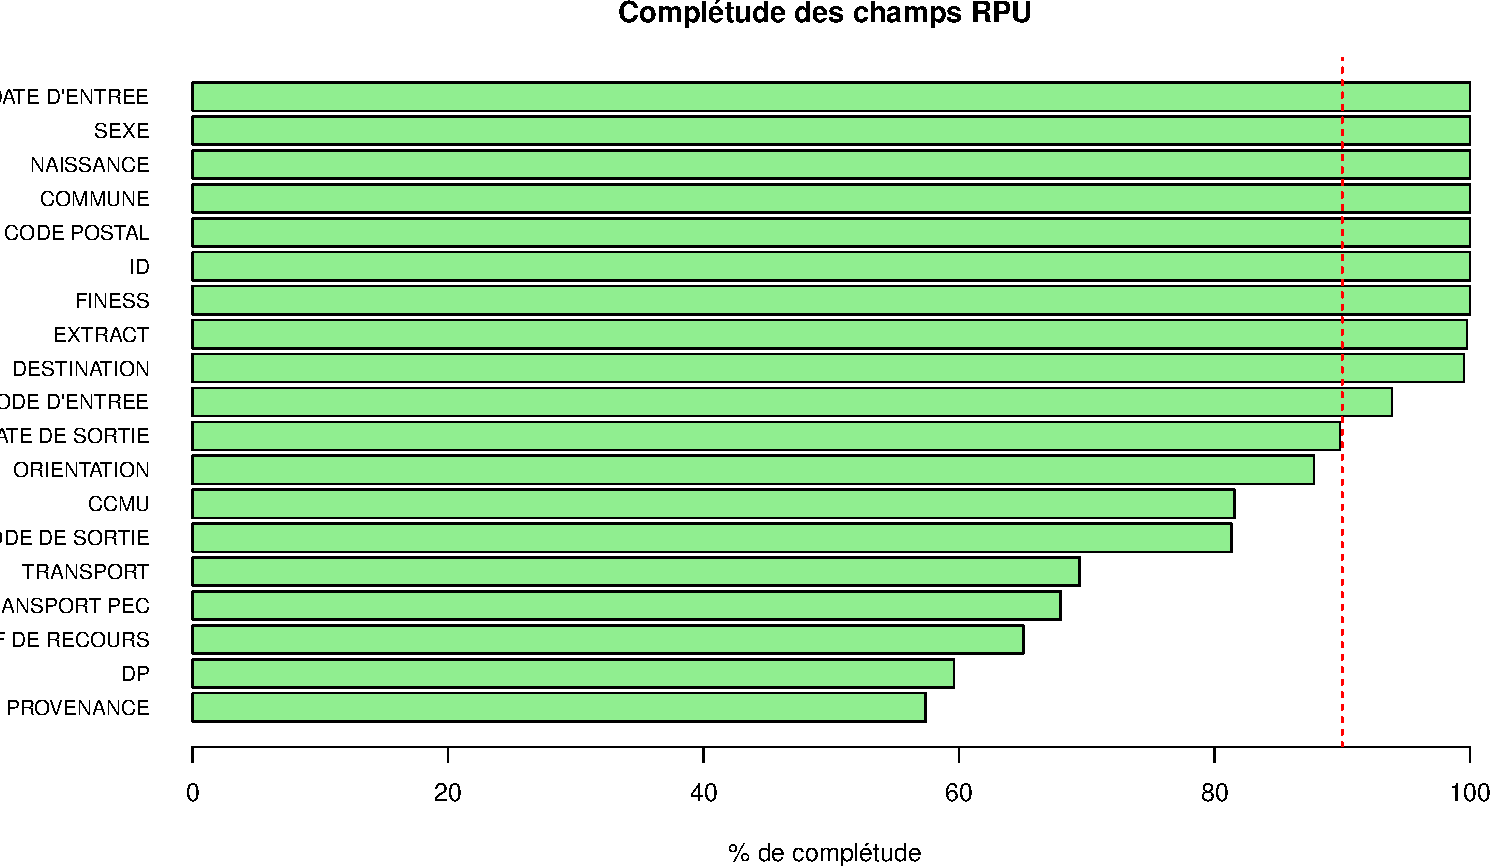
\includegraphics{rapport2014_V4_files/figure-latex/completude-1.pdf}
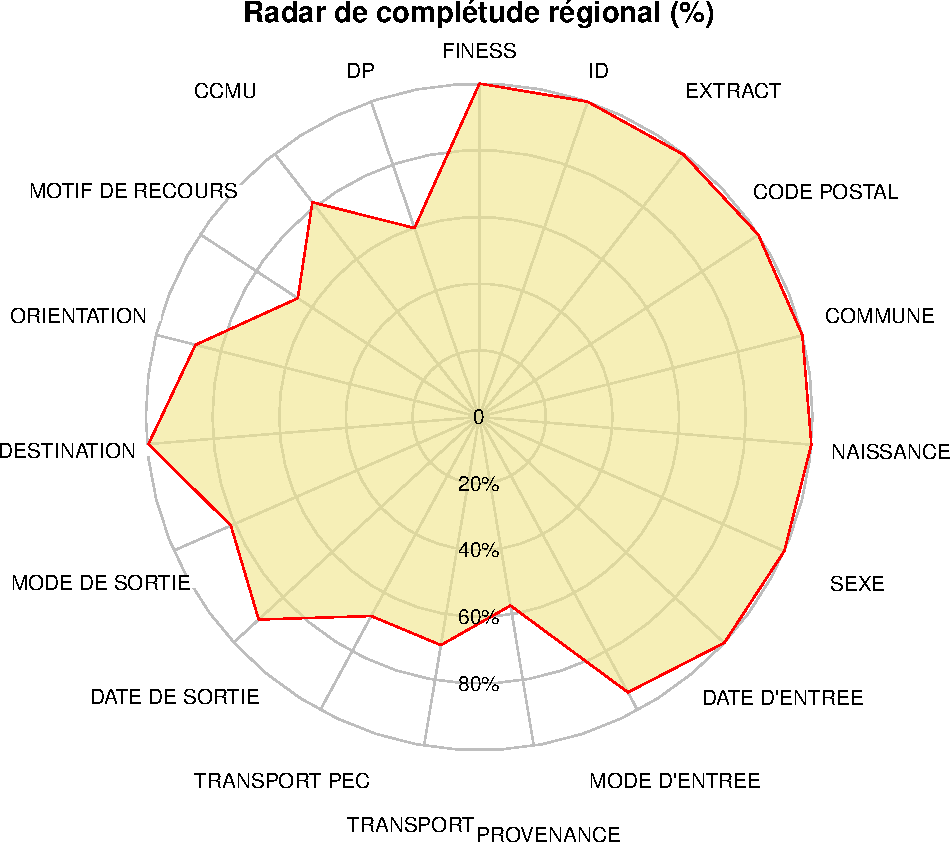
\includegraphics{rapport2014_V4_files/figure-latex/completude-2.pdf}

\section{Les chiffres clés de l'activité des services
d'urgences}\label{les-chiffres-cles-de-lactivite-des-services-durgences}

\subsection{Recueil des données}\label{recueil-des-donnees}

\begin{itemize}
\itemsep1pt\parskip0pt\parsep0pt
\item
  Nombre de passages dans l'année {[}C{]}: 40 509 RPU
\item
  Moyenne quotidienne de passages {[}C{]}: 1 307 RPU
\item
  \%(N) d'évolution par rapport à année N-1 {[}C{]}: 12 \%.
\item
  \% d'évolution moyenne sur les 5 dernières années (méthode calcul :
  moyenne des évolutions constatées entre chaque année)
\item
  Données renseignées (données à partir desquelles tout le reste de
  l'analyse sera effectuée)

  \begin{itemize}
  \itemsep1pt\parskip0pt\parsep0pt
  \item
    Nombre de RPU transmis: 40 509 RPU
  \item
    Exhaustivité du recueil : Nb RPU transmis / Nb de passages déclarés
    8,2 \% (NOTE le nombre de passages déclarés est celui indiqué par
    les données SAE 2013)
  \end{itemize}
\end{itemize}

\subsection{PATIENTS}\label{patients}

\subsubsection{SEXE}\label{sexe}

\begin{itemize}
\itemsep1pt\parskip0pt\parsep0pt
\item
  \%(N) Femme {[}C{]}: 49.39 \% (19 997)
\item
  \%(N) Homme {[}C{]}: 50.61 \% (20 488)
\item
  Sex ratio: 1.02
\item
  Taux de masculinité: 0.51
\end{itemize}

\subsubsection{Age}\label{age}

\begin{itemize}
\item
  age moyen{[}C{]}: 37.13 ans.
\item
  age moyen des hommes {[}S{]}: 35.34 ans.
\item
  age moyen des femmes {[}S{]}: 38.99 ans.
\item
  \% (N) \textless{} 1 an {[}C{]}: 1991 (4.92 \%)
\item
  \%(N) \textless{} 15 ans {[}C{]}: 11184 (27.61 \%)
\item
  \%(N) \textless{} 18 ans {[}C{]}: 12769 (31.52 \%)
\item
  \%(N) \textgreater{}= 75 ans {[}C{]}: 5671 (14 \%)
\item
  Pyramide des ages:
\end{itemize}

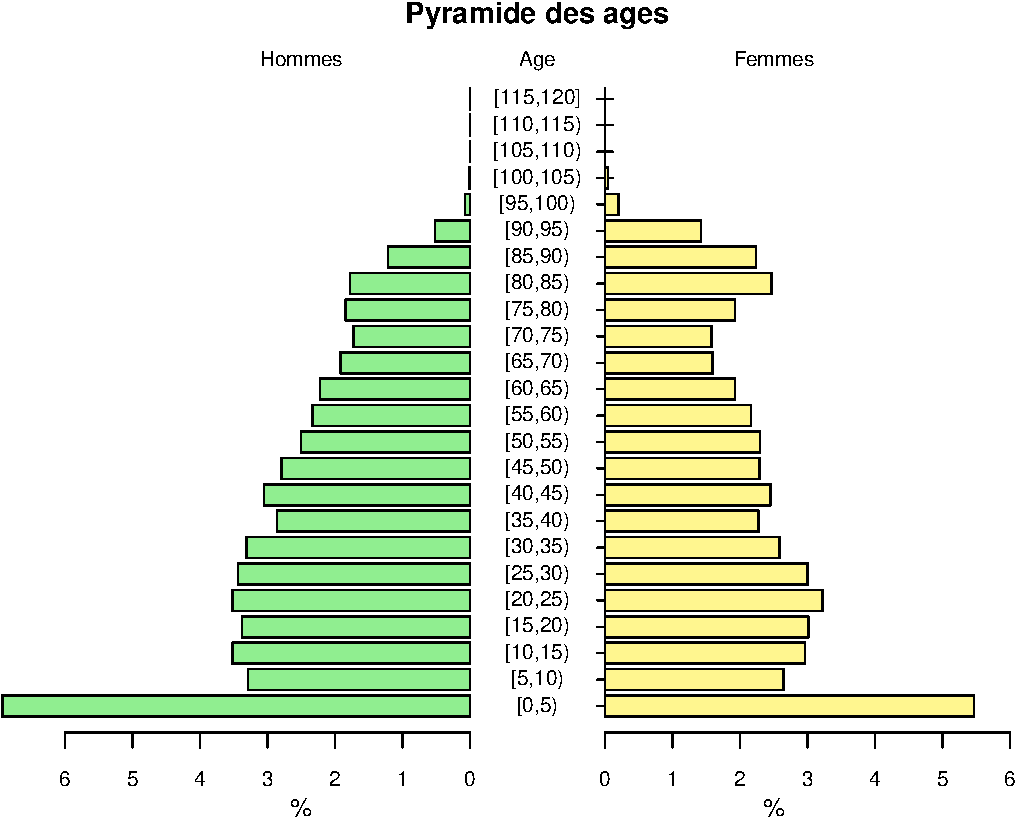
\includegraphics{rapport2014_V4_files/figure-latex/pyramide-1.pdf}

\begin{verbatim}
## [1] 5.1 4.1 4.1 2.1
\end{verbatim}

\subsubsection{Taux de recours (définition FEDORU) régional aux
urgences.
{[}S{]}}\label{taux-de-recours-definition-fedoru-regional-aux-urgences.-s}

Utilisation des données INSEE qui collent le plus à la période d'étude
(projections ou données consolidées)

\subsubsection{\% de patients ne venant pas de la région (étranger
compris)}\label{de-patients-ne-venant-pas-de-la-region-etranger-compris}

\subsection{ARRIVÉE}\label{arrivee}

\subsubsection{Horaires de passage}\label{horaires-de-passage}

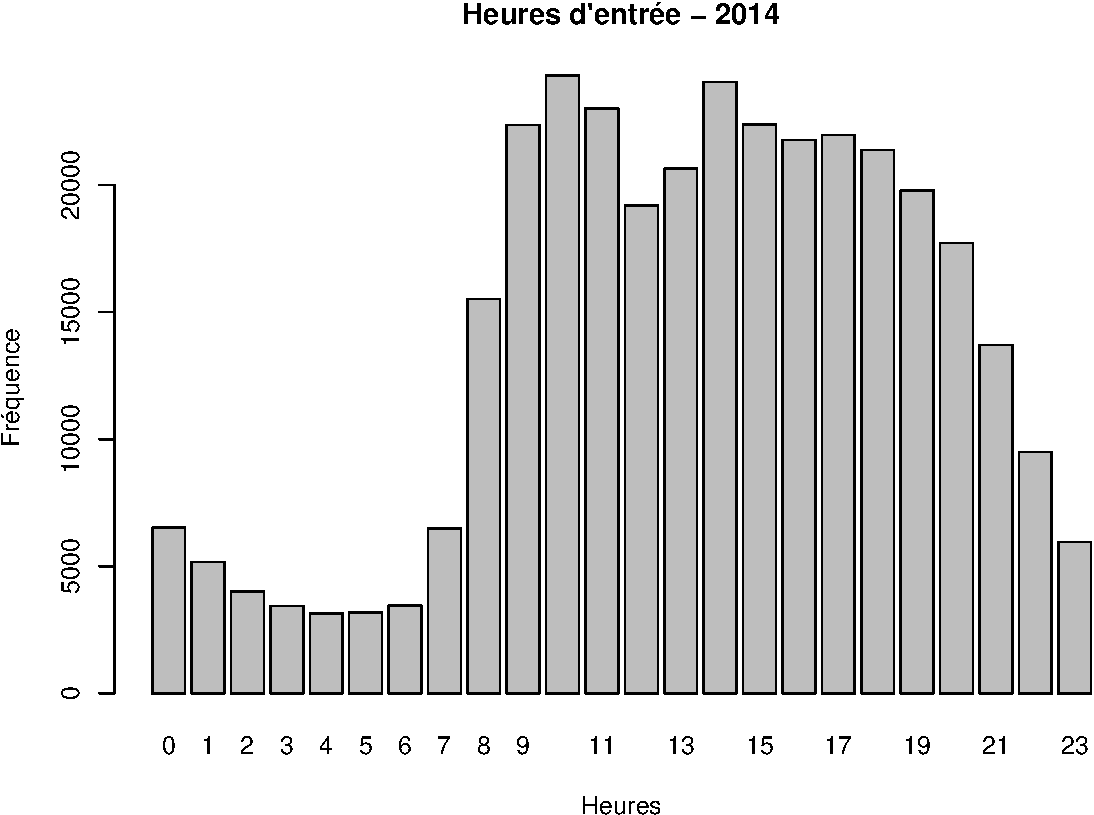
\includegraphics{rapport2014_V4_files/figure-latex/horaires-1.pdf}

\begin{itemize}
\itemsep1pt\parskip0pt\parsep0pt
\item
  \% passages nuit {[}C{]}: 23.61 \% (N = 8561)
\item
  \% passages nuit profonde {[}C{]}: 11.27 \% (N = 4088)
\item
  \% passages en horaire de PDS
\end{itemize}

\subsubsection{Moyens d'arrivée}\label{moyens-darrivee}

\begin{itemize}
\itemsep1pt\parskip0pt\parsep0pt
\item
  \textbf{\%(N) d'arrivée personnel} {[}S{]}: 68.91 \% (N = 19 913)
\item
  \textbf{\%(N) d'arrivée SMUR} {[}S{]}: 1.06 \% (N = 305)
\item
  \textbf{\%(N) d'arrivée VSAB} {[}S{]}: 10.3 \% (N = 2 977)
\item
  \textbf{\%(N) d'arrivée Ambulance} {[}S{]}: 19.13 \% (N = 5 527)
\end{itemize}

NB : commentaire possible pour expliquer que la somme des 4 pourcentages
ci dessus ne fait pas 100 \%

\subsubsection{Gravité (CCMU)}\label{gravite-ccmu}

\begin{itemize}
\itemsep1pt\parskip0pt\parsep0pt
\item
  \textbf{\%(N) CCMU 1 et 2} {[}C{]}: 84.16\% (n = 26549)
\item
  \textbf{\%(N) CCMU 4 et 5} {[}C{]}: 1.38\% (n = 434)
\end{itemize}

DIAGNOSTIC PRINCIPAL

\% Médico-chirurgical \% Traumatologique \% Psychiatrique \%
Toxicologique \% Autres recours

\subsubsection{Durées de passage}\label{durees-de-passage}

\begin{itemize}
\item
  durée moyenne de passage 174 mn.
\item
  écart-type: 173.5 mn.
\item
  médiane: 123 mn.
\item
  nombre de passages \textgreater{} 4 heures: 8465 (23.61 \%).
\item
  nombre de passages inférieurs ou égaux à 4 heures: 27385 (76.39 \%).
\item
  Lors d'une hospitalisation post-urgences (hospitalisation = mutation +
  transfert)
\item
  Lors d'un retour au domicile
\end{itemize}

\subsubsection{MODE DE SORTIE}\label{mode-de-sortie}

\begin{itemize}
\itemsep1pt\parskip0pt\parsep0pt
\item
  \% (N) de retour à domicile: 75.36 \% (N = 21 497)
\item
  \% (N) Hospitalisation: 24.64 \% (N = 7 029)
\item
  \% (N) Mutation: 23.1 \% (N = 6 590)
\item
  \% (N) Transfert: 1.54 \% (N = 439)
\end{itemize}

\section{Les chiffres clés de l'activité des
SAMU}\label{les-chiffres-cles-de-lactivite-des-samu}

(à partir des données SRVA ``officielles'')

\begin{itemize}
\itemsep1pt\parskip0pt\parsep0pt
\item
  Nombre de dossiers de régulation médicale (DRM)
\item
  Nombre de SMUR :

  \begin{itemize}
  \itemsep1pt\parskip0pt\parsep0pt
  \item
    dont primaires
  \end{itemize}
\item
  Nombre d'ambulances privées à la demande du SAMU
\end{itemize}

\section{Les chiffres clés de l'activité pédiatrique des services
d'urgences (moins de 18
ans)}\label{les-chiffres-cles-de-lactivite-pediatrique-des-services-durgences-moins-de-18-ans}

\section{Les chiffres clés de l'activité gériatrique des services
d'urgences (plus de 75
ans)}\label{les-chiffres-cles-de-lactivite-geriatrique-des-services-durgences-plus-de-75-ans}

\subsection{RECUEIL DES DONNÉES}\label{recueil-des-donnees-1}

\begin{itemize}
\itemsep1pt\parskip0pt\parsep0pt
\item
  Nombre de passages dans l'année: 5393
\item
  Moyenne quotidienne de passage: 173.97 passages/j
\item
  Taux d'urgences gériatriques (Nb RPU Géria/ Nb RPU global)*100: 13.31
  \%
\item
  TODO: \% d'évolution par rapport à l'année N-1(données SAE pour ceux
  qui n'ont pas d'historique RPU fiable et permettant la comparaison,
  préciser l'origine des données)
\end{itemize}

\subsection{PATIENTS}\label{patients-1}

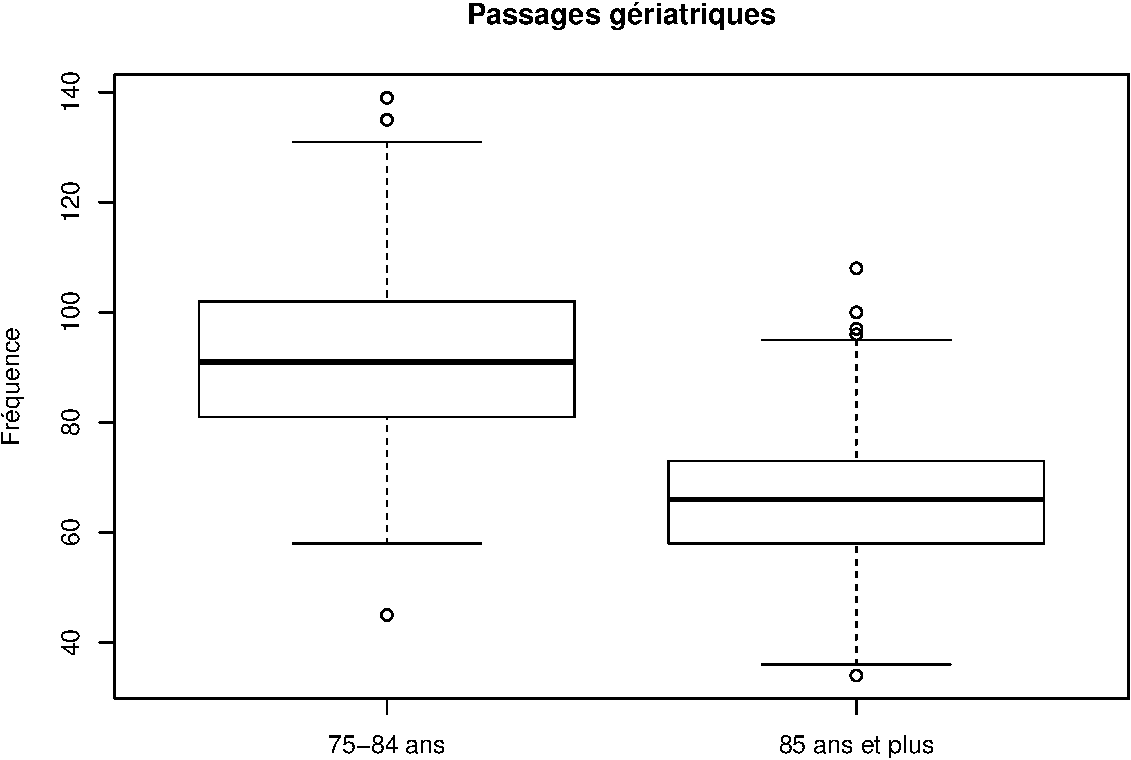
\includegraphics{rapport2014_V4_files/figure-latex/sexe75-1.pdf}

\section{Les chiffres clés de l'activité AVC des services
d'urgences}\label{les-chiffres-cles-de-lactivite-avc-des-services-durgences}

\section{ANNEXES}\label{annexes}

\subsection{ANNEXE 1 : Définitions}\label{annexe-1-definitions}

\subsection{ANNEXE 2 : Diagramme de complétude des
RPU}\label{annexe-2-diagramme-de-completude-des-rpu}

\subsection{ANNEXE 3 : Calcul du TARRU}\label{annexe-3-calcul-du-tarru}

\end{document}
